\documentclass[twoside]{article}
\usepackage[utf8]{inputenc}
\usepackage[ngerman]{babel}
\usepackage{libertine}
\usepackage[dvipsnames]{xcolor}
\usepackage[a4paper]{geometry}
\usepackage{pdfpages}
\usepackage{parskip}
\usepackage{amsmath, amsthm, amssymb, commath, mathtools}
\usepackage{cancel}
\usepackage{physics}
\usepackage[version=4]{mhchem}
\usepackage{nicefrac}
\usepackage{booktabs}
\usepackage{tabularx}
\usepackage{tabu}
\usepackage{enumitem}
\usepackage{graphicx}
\graphicspath{{./plots/}{./images/}}
\usepackage{wrapfig}
\definecolor{capblue}{HTML}{00709B}
\usepackage[margin=1cm,font={small},labelfont={color=capblue}]{caption}
\usepackage{subcaption}
\usepackage{float}
\usepackage{minted}
\usepackage{appendix}
\usepackage{icomma}
\usepackage{multirow}
\usepackage{multicol}
\usepackage{footmisc}
\usepackage[separate-uncertainty=true]{siunitx}
\sisetup{locale = DE}
\usepackage{tcolorbox}

\usepackage{ccicons}

\usepackage{csquotes}
\MakeOuterQuote{"}
\renewcommand{\ttdefault}{cmtt}

\usepackage{hyperref}
\usepackage{bookmark}
% https://tex.stackexchange.com/a/33701
\makeatletter
    \newcommand{\nonum}[0]{%
        \let\@oldseccntformat\@seccntformat %
        \renewcommand\@seccntformat[1]{}%
        }
    \newcommand{\resnum}[0]{\let\@seccntformat\@oldseccntformat}
\makeatother

\usepackage{chngcntr}
\counterwithin{figure}{section}
\counterwithin{table}{section}

\usepackage[style=iso-authoryear,sortcites=true,sorting=nyt,backend=biber,language=ngerman,natbib=true,sortlocale=de_DE]{biblatex}
\addbibresource{references.bib}
\newcommand{\mkbibbracketscol}[1]{\textcolor{gray}{\mkbibbrackets{#1}}}
\DeclareCiteCommand{\cite}[\mkbibbracketscol]
  {\usebibmacro{prenote}}
  {\usebibmacro{citeindex}%
   \usebibmacro{cite}}
  {\multicitedelim}
  {\usebibmacro{postnote}}

\DeclareCiteCommand{\parencite}[\mkbibbracketscol]
  {\usebibmacro{prenote}}
  {\usebibmacro{citeindex}%
   \usebibmacro{cite}}
  {\multicitedelim}
  {\usebibmacro{postnote}}


\DeclareCiteCommand{\cbx@textcite}[\textcolor{gray}]
  {\usebibmacro{textcite:init}}
  {\usebibmacro{citeindex}%
   \usebibmacro{textcite}}
  {}
  {\usebibmacro{textcite:postnote}}

\DefineBibliographyStrings{ngerman}{%
    bibliography    = {Literaturverzeichnis},
    andothers       = {u.\,a.\adddot}
}

\let\realcitep\citep
\renewcommand*{\citep}[1]{{\footnotesize\realcitep{#1}}}

\newcommand{\versuch}[0]{FHV}
\newcommand{\versuchLang}[0]{Franck-Hertz Versuch}

\hypersetup{
	pdftitle={P3B -- \versuch{} Auswertung},
	pdfauthor={Yudong Sun},
	bookmarksnumbered=true,
	bookmarksopen=true,
	bookmarksopenlevel=2,
	pdfstartview=Fit,
	pdfpagemode=UseOutlines,
	colorlinks=true,
	linkcolor=black,
	filecolor=magenta,      
	urlcolor=blue,
    citecolor=gray
}
\urlstyle{same}

\title{\versuch{} -- \versuchLang \\ Auswertung}
\author{Yudong Sun\\Gruppe L8}

\usepackage{fancyhdr}
\pagestyle{fancy}
\fancyhf{}
\fancyhead[RO]{Yudong Sun}
\fancyhead[LO]{Auswertung -- \versuch}
\fancyhead[LE]{Yudong Sun}
\fancyhead[RE]{Auswertung -- \versuch}
\cfoot{\thepage}

% Custom Defs
\newcommand*{\ra}[1]{\renewcommand{\arraystretch}{#1}}
\newcommand*{\maxi}[1]{\text{max}\left(#1\right)}
\newcommand*{\mini}[1]{\text{min}\left(#1\right)}
\newcommand*{\todo}[1]{\textcolor{red}{TODO: #1}}
\newcommand*{\iu}[1]{\textit{\underline{#1}}}
\newcommand*{\gnuplot}[0]{\texttt{gnuplot}}
\newcommand*{\captionbr}[0]{\\\rule{\textwidth}{0pt}\\\vspace{-\baselineskip}}
\newcommand*{\sigfig}[1]{\hspace{0.5cm}\text{(#1 sig. Zif.)}}
\newcommand*{\pbrace}[1]{\left(#1\right)}
\newcommand*{\sbrace}[1]{\left[#1\right]}
\newcommand*{\bDelta}[1]{\pbrace{\Delta #1}}
\newcommand*{\overbar}[1]{\overline{\raisebox{0pt}[1.2\height]{$#1$}}} % https://tex.stackexchange.com/a/87615
\newenvironment{beispiel}
    {\begin{tcolorbox}[title=Beispielrechnung]}
    {\end{tcolorbox}}

\newcommand*{\realzahl}[0]{\mathbb{R}}
\newcommand*{\natzahl}[0]{\mathbb{N}}
\newcommand*{\ratzahl}[0]{\mathbb{Q}}
\newcommand*{\intzahl}[0]{\mathbb{Z}}
\newcommand*{\boolzahl}[0]{\mathbb{B}}

\newcommand*{\question}[1]{\textit{\textcolor{Magenta}{#1}}}

% \addto\captionsngerman{
%     \let\oldfigname\figurename
%     \renewcommand{\figurename}{[\oldfigname}
%     \let\oldthefig\thefigure
%     \renewcommand{\thefigure}{\oldthefig]}
% } % https://tex.stackexchange.com/a/17490
% https://tex.stackexchange.com/a/101624 new line in caption

% Gaußsche Fehler Erzeuger
\makeatletter
    \newcommand{\gausserror}[2]{% \gausserror{G}{faktoren}
        \sqrt{%
            \@tempswafalse
            \@for\factor:=#2
            \do{
                \if@tempswa+%
                \else%
                    \@tempswatrue%
                \fi%
                \left(\pdv{#1}{\factor}\Delta\factor\right)^2%
            }%
        }
    }
\makeatother
% https://tex.stackexchange.com/a/59912
% https://riptutorial.com/latex/example/28657/loops---repeating-things

% Add quad
\makeatletter
    \newcommand{\addquad}[1]{% \gausserror{G}{faktoren}
        \sqrt{%
            \@tempswafalse
            \@for\factor:=#1
            \do{
                \if@tempswa+%
                \else%
                    \@tempswatrue%
                \fi%
                \left(\Delta\factor\right)^2%
            }%
        }
    }
\makeatother

% rej quad
\makeatletter
    \newcommand{\relquad}[1]{% \gausserror{G}{faktoren}
        \sqrt{%
            \@tempswafalse
            \@for\factor:=#1
            \do{
                \if@tempswa+%
                \else%
                    \@tempswatrue%
                \fi%
                \left(\frac{\Delta\factor}{\factor}\right)^2%
            }%
        }
    }
\makeatother

\newcommand*{\ub}[1]{\underbracket[0.1ex]{#1}}
\newcommand*{\ob}[1]{\overbracket[0.1ex]{#1}}
\newcommand*{\brc}[2]{\mathrlap{\ub{\phantom{#1}}_{#2}}#1}
\newcommand*{\brd}[2]{\mathrlap{\ob{\phantom{#1}}^{#2}}#1}

% / Custom Defs

\begin{document}

\maketitle

% Einstellungen
\nonum
\numberwithin{equation}{section}
% / Einstellungen

\section{Teilversuch 1: Bragg Reflexion von Röntgenstrahlung des Molybdän an einem \ce{NaCl}-Einkristall}
	\begin{figure}[!ht]
		\centering
		\begin{subfigure}{0.48\textwidth}
			\centering
			\includegraphics[width=\textwidth]{images/tv1-aufbau.jpg}
			\caption{Röntgengerät}
			% \vspace{0.5\baselineskip}
			\label{fig:tv1-1}
		\end{subfigure}
		\begin{subfigure}{0.48\textwidth}
			\centering
			\includegraphics[width=\textwidth]{images/tv1-aufbau2.jpg}
			\caption{Probetisch mit \ce{NaCl}-Einkristall und detektor}
			% \vspace{0.5\baselineskip}
			\label{fig:tv1-2}
		\end{subfigure}
	    \caption{Aufbau von Teilversuch 1}
	\end{figure}
	Wir berechnen zunächst aus unseren $\beta$-Winkeln die entsprechende Wellenlängen. Es gilt:
	\begin{align}
		n\lambda = 2d\sin\beta \notag \\
		\Rightarrow \lambda &= \frac{2d\sin\beta}{n} \\
		\Delta\lambda &= \gausserror{\lambda}{\beta} = \abs{\frac{2d\Delta\beta}{n}\cos{\beta}}
	\end{align}
	wobei alle Winkel in Radian sind. Alle Rechnung erfolgen in LibreOffice Calc.
	\pagebreak
	Um den Mittelwert und Fehler des Mittelwertes zu berechnen, verwenden wir die gerundeten Werten und die Funktion \texttt{AVERAGE} bzw. die Formel:
	\begin{align}
		\Delta \overline{\lambda} = \frac{\addquad{\lambda_1, \lambda_2, \lambda_3}}{3} \label{eqn:tv1-error}
	\end{align}
	wobei der Zähler mithilfe der Funktion \texttt{SUMSQ} in LibreOffice Calc gerechnet ist. 

	Da $n = 3$ noch ziemlich klein ist, ist es nicht sinnvoll die Formel für die Standardabweichung zu verwenden. Die Formel für die Standardabweichung geht von einer gaußschen Verteilung aus, was wir hier nicht gewährleisten können. Wir verwenden somit direkte Fehlerfortpflanzung. 

	Wir erhalten somit:
	\begin{center}
		\vspace{\parskip}
		\begin{tabular}{lrrrr}
			\toprule
			& \multicolumn{2}{c}{$K_\alpha$} & \multicolumn{2}{c}{$K_\beta$} \\
			\cmidrule(lr){2-3} \cmidrule(lr){4-5} % https://tex.stackexchange.com/q/180368
			$n$ & $\beta/\si{\degree}$ & $\lambda/\si{\pico\meter}$ & $\beta/\si{\degree}$ & $\lambda/\si{\pico\meter}$ \\
			\midrule
			$1$ & \num{7.26(12)} & \num{71.3(12)} & \num{6.46(12)} & \num{63.5(12)} \\
			$2$ & \num{14.64(12)} & \num{71.3(6)} & \num{12.96(14)} & \num{63.2(7)} \\
			$3$ & \num{22.24(14)} & \num{71.2(5)} & \num{19.7(8)} & \num{63.38(25)} \\
			\cmidrule(lr){3-3} \cmidrule(lr){5-5}
			& (Mittelwert) & \num{71.3(5)} & (Mittelwert) & \num{63.4(5)} \\
			& ($\lambda_\text{Lit}$) & \num{71.08} & ($\lambda_\text{Lit}$) & \num{63.09} \\
			\bottomrule
		\end{tabular}
		\vspace{\parskip}
	\end{center}
	Die experimenlle Werten stimmen mit der Literaturwerten überein.


\section{Teilversuch 2: Kugelflächenfunktionen im Spärischen Resonator}
	\subsection{Teilversuch 2a: Zuordnung der Legendrepolynome durch Bestimmung der Nullstellen}
		Alle Frequenzen sind mittels digitale Signalgenerator eingestellt, somit ist keine Unsicherheit gegeben. Man sieht aber auf dem Oszilloskop schon einige Abweichungen/Geräusch von Signal.

		Eine Fehler von $\Delta V = \pm \SI{0.002}{\volt}$ ist abgeschätzt.
		\begin{center}
			\begin{tabular}{llrrr}
				\toprule
				\multicolumn{2}{r}{$f$/\si{\hertz}} & \num{3,663} & \num{4,950} & \num{6,190} \\
				$\alpha$/\si{\degree} & $\theta$/\si{\degree} & Spannung/\si{\volt} & Spannung/\si{\volt} & Spannung/\si{\volt}  \\
				\midrule
				\num{180} & \num{180} & \num{0,373} & \num{0,539} & \num{-0,303} \\
				\num{170} & \num{172,933425610738} & \num{0,356} & \num{0,528} & \num{-0,279} \\
				\num{160} & \num{165,893955739434} & \num{0,331} & \num{0,474} & \num{-0,211} \\
				\num{150} & \num{158,909418821001} & \num{0,295} & \num{0,375} & \num{-0,103} \\
				\num{140} & \num{152,009109282217} & \num{0,243} & \num{0,244} & \num{0,011} \\
				\num{130} & \num{145,224563330281} & \num{0,189} & \num{0,091} & \num{0,103} \\
				\num{120} & \num{138,590377890729} & \num{0,138} & \num{-0,052} & \num{0,169} \\
				\num{110} & \num{132,145070558482} & \num{0,031} & \num{-0,151} & \num{0,187} \\
				\num{100} & \num{125,93195832035} & \num{0,031} & \num{-0,225} & \num{0,169} \\
				\num{90} & \num{120} & \num{0,042} & \num{-0,259} & \num{0,117} \\
				\num{80} & \num{114,404497337886} & \num{0,780} & \num{-0,269} & \num{0,046} \\
				\num{70} & \num{109,207479725344} & \num{-0,128} & \num{-0,236} & \num{0,029} \\
				\num{60} & \num{104,47751218593} & \num{-0,105} & \num{-0,185} & \num{-0,071} \\
				\num{50} & \num{100,288585136763} & \num{-0,182} & \num{-0,119} & \num{-0,091} \\
				\num{40} & \num{96,7177134641804} & \num{-0,167} & \num{-0,055} & \num{-0,085} \\
				\num{30} & \num{93,8409657162581} & \num{-0,189} & \num{-0,099} & \num{-0,065} \\
				\num{20} & \num{91,7279410723505} & \num{-0,202} & \num{-0,069} & \num{-0,040} \\
				\num{10} & \num{90,4352300024699} & \num{-0,205} & \num{-0,099} & \num{-0,030} \\
				\num{0} & \num{90} & \num{-0,210} & \num{-0,112} & \num{0,032} \\
				\bottomrule
			\end{tabular}
		\end{center}		
		Insbesondere es ist während der Plotting auffällig, dass die Vorzeichen für $f = \SI{4.950}{\hertz}$ und $\SI{6.190}{\hertz}$ andersrum sein sollten, also sind die Messwerte während der Kurveanpassung entsprechend angepasst. 

		Aus Gleichung (43) der Anleitung gilt:
		\begin{align}
			\theta &= \arccos\left(\frac{1}{2}\cos(\alpha) - \frac{1}{2}\right) \\
			\Rightarrow \Delta \theta &= \gausserror{\theta}{\alpha} = \frac{\sin(\alpha)\Delta \alpha}{\sqrt{-\cos^2(\alpha) + 2 \cos(\alpha) + 3}}
		\end{align}
		wobei alle Winkel in Formel in Radian sind. Somit ergibt sich aus $\Delta\alpha = \pm\SI{1}{\degree}$:
		\begin{center}
			\begin{tabular}{l|r|r|rrr}
				\toprule
				Frequenz $f$/\si{\hertz} & \num{3.663} & \num{4.950} & \num{6.190} & \num{6.190} & \num{6.190} \\
				\midrule
				Nullstelle $\theta$/\si{\degree} & \num{125.3(7)} & \num{141.2(7)} & \num{90.1(6)} & \num{110.2(7)} & \num{152.7(7)} \\
				Nullstelle $\theta_\text{Lit}$/\si{\degree} & \num{125.26} & \num{140.77} & ? & \num{109.88} & \num{149.44} \\
				\bottomrule				
			\end{tabular}
		\end{center}
		Alle Rechnungen erfolgt in LibreOffice Calc. 

		Die zugeordnete Legendrepolynome haben $l-m$ Nullstellen. Aus dem spätere Teilversuch 2b wissen wir, dass es hier um $m = 0$ handelt. Wir vergleichen die Werte oben mit der Literaturwerte auf Seite 32 der Anleitung und erhalten:
		\begin{center}
			\begin{tabular}{lrrr}
				\toprule
				Frequenz $f$/\si{\hertz} & \num{3.663} & \num{4.950} & \num{6.190} \\
				\midrule
				Ordnung $l$ & $2$ & $3$ & $4$\\
				\bottomrule				
			\end{tabular}
		\end{center}
		Die Nullstelle bei $\theta = \SI{90.1(6)}{\degree}$ ist anscheinend eine Fehlmessung, weil es für $l = 4$ keine Nullstelle bei diesem Winkel $\theta$ gibt. Das könnte daran liegen, dass $\alpha = \SI{5(1)}{\degree}$ sehr nah am Rand der Skala ist und dass der Aufbau die Legendrepolynome nicht perfekt simulieren kann. Die Ordnungen sind auch im Laborprotokoll zum Teilversuch 2b vermerkt.

		Für die Kurveanpassung brauchen wir noch die Fehlerbalken:
		\begin{align}
			\cos(\theta) &= \frac{1}{2}\cos(\alpha) - \frac{1}{2} \\
			\Rightarrow \Delta \cos(\theta) &= \gausserror{\cos(\theta)}{\alpha} = \abs{\frac{-\sin(\alpha)\Delta\alpha}{2}}
		\end{align}
		Wir passen nun die Kurven an in \gnuplot{} (Siehe Appendix \ref{appdx:tv2a}):
		\begin{center}
			\begin{tabular}{lll}
				\toprule
				Ordnung $l$ & Fit-Funktion & Anfangswerte \\
				\midrule
				$2$ & $Ax^2 + B$  & $A = 1.5, B = -0.5$ \\
				$3$ & $Cx^3 + Dx$ & $C = 2.5, D = -1.5$ \\
				$4$ & $Ex^4 + Fx^2 + G$  & $E = \nicefrac{35}{8}, F = -\nicefrac{30}{8}, G = \nicefrac{3}{8}$ \\
				\bottomrule
			\end{tabular}
		\end{center}
		\newpage
		\begin{figure}[!ht]
		    \centering
		    % \vspace{-1em}
		    % https://tex.stackexchange.com/a/98142
		    \resizebox{\textwidth}{!}{% GNUPLOT: LaTeX picture with Postscript
\begingroup
  \makeatletter
  \providecommand\color[2][]{%
    \GenericError{(gnuplot) \space\space\space\@spaces}{%
      Package color not loaded in conjunction with
      terminal option `colourtext'%
    }{See the gnuplot documentation for explanation.%
    }{Either use 'blacktext' in gnuplot or load the package
      color.sty in LaTeX.}%
    \renewcommand\color[2][]{}%
  }%
  \providecommand\includegraphics[2][]{%
    \GenericError{(gnuplot) \space\space\space\@spaces}{%
      Package graphicx or graphics not loaded%
    }{See the gnuplot documentation for explanation.%
    }{The gnuplot epslatex terminal needs graphicx.sty or graphics.sty.}%
    \renewcommand\includegraphics[2][]{}%
  }%
  \providecommand\rotatebox[2]{#2}%
  \@ifundefined{ifGPcolor}{%
    \newif\ifGPcolor
    \GPcolortrue
  }{}%
  \@ifundefined{ifGPblacktext}{%
    \newif\ifGPblacktext
    \GPblacktexttrue
  }{}%
  % define a \g@addto@macro without @ in the name:
  \let\gplgaddtomacro\g@addto@macro
  % define empty templates for all commands taking text:
  \gdef\gplbacktext{}%
  \gdef\gplfronttext{}%
  \makeatother
  \ifGPblacktext
    % no textcolor at all
    \def\colorrgb#1{}%
    \def\colorgray#1{}%
  \else
    % gray or color?
    \ifGPcolor
      \def\colorrgb#1{\color[rgb]{#1}}%
      \def\colorgray#1{\color[gray]{#1}}%
      \expandafter\def\csname LTw\endcsname{\color{white}}%
      \expandafter\def\csname LTb\endcsname{\color{black}}%
      \expandafter\def\csname LTa\endcsname{\color{black}}%
      \expandafter\def\csname LT0\endcsname{\color[rgb]{1,0,0}}%
      \expandafter\def\csname LT1\endcsname{\color[rgb]{0,1,0}}%
      \expandafter\def\csname LT2\endcsname{\color[rgb]{0,0,1}}%
      \expandafter\def\csname LT3\endcsname{\color[rgb]{1,0,1}}%
      \expandafter\def\csname LT4\endcsname{\color[rgb]{0,1,1}}%
      \expandafter\def\csname LT5\endcsname{\color[rgb]{1,1,0}}%
      \expandafter\def\csname LT6\endcsname{\color[rgb]{0,0,0}}%
      \expandafter\def\csname LT7\endcsname{\color[rgb]{1,0.3,0}}%
      \expandafter\def\csname LT8\endcsname{\color[rgb]{0.5,0.5,0.5}}%
    \else
      % gray
      \def\colorrgb#1{\color{black}}%
      \def\colorgray#1{\color[gray]{#1}}%
      \expandafter\def\csname LTw\endcsname{\color{white}}%
      \expandafter\def\csname LTb\endcsname{\color{black}}%
      \expandafter\def\csname LTa\endcsname{\color{black}}%
      \expandafter\def\csname LT0\endcsname{\color{black}}%
      \expandafter\def\csname LT1\endcsname{\color{black}}%
      \expandafter\def\csname LT2\endcsname{\color{black}}%
      \expandafter\def\csname LT3\endcsname{\color{black}}%
      \expandafter\def\csname LT4\endcsname{\color{black}}%
      \expandafter\def\csname LT5\endcsname{\color{black}}%
      \expandafter\def\csname LT6\endcsname{\color{black}}%
      \expandafter\def\csname LT7\endcsname{\color{black}}%
      \expandafter\def\csname LT8\endcsname{\color{black}}%
    \fi
  \fi
    \setlength{\unitlength}{0.0500bp}%
    \ifx\gptboxheight\undefined%
      \newlength{\gptboxheight}%
      \newlength{\gptboxwidth}%
      \newsavebox{\gptboxtext}%
    \fi%
    \setlength{\fboxrule}{0.5pt}%
    \setlength{\fboxsep}{1pt}%
    \definecolor{tbcol}{rgb}{1,1,1}%
\begin{picture}(8640.00,7200.00)%
    \gplgaddtomacro\gplbacktext{%
      \csname LTb\endcsname%%
      \put(946,704){\makebox(0,0)[r]{\strut{}$-0,6$}}%
      \put(946,1288){\makebox(0,0)[r]{\strut{}$-0,5$}}%
      \put(946,1871){\makebox(0,0)[r]{\strut{}$-0,4$}}%
      \put(946,2454){\makebox(0,0)[r]{\strut{}$-0,3$}}%
      \put(946,3038){\makebox(0,0)[r]{\strut{}$-0,2$}}%
      \put(946,3621){\makebox(0,0)[r]{\strut{}$-0,1$}}%
      \put(946,4205){\makebox(0,0)[r]{\strut{}$0$}}%
      \put(946,4789){\makebox(0,0)[r]{\strut{}$0,1$}}%
      \put(946,5372){\makebox(0,0)[r]{\strut{}$0,2$}}%
      \put(946,5955){\makebox(0,0)[r]{\strut{}$0,3$}}%
      \put(946,6539){\makebox(0,0)[r]{\strut{}$0,4$}}%
      \put(1078,484){\makebox(0,0){\strut{}$-1$}}%
      \put(2511,484){\makebox(0,0){\strut{}$-0,8$}}%
      \put(3944,484){\makebox(0,0){\strut{}$-0,6$}}%
      \put(5377,484){\makebox(0,0){\strut{}$-0,4$}}%
      \put(6810,484){\makebox(0,0){\strut{}$-0,2$}}%
      \put(8243,484){\makebox(0,0){\strut{}$0$}}%
    }%
    \gplgaddtomacro\gplfronttext{%
      \csname LTb\endcsname%%
      \put(209,3621){\rotatebox{-270}{\makebox(0,0){\strut{}Amplitude $A$ ($\si{\volt}$)}}}%
      \put(4660,154){\makebox(0,0){\strut{}$\cos(\theta/\si{\degree})$}}%
      \csname LTb\endcsname%%
      \put(4949,1317){\makebox(0,0)[r]{\strut{}$l = 2$}}%
      \csname LTb\endcsname%%
      \put(4949,1097){\makebox(0,0)[r]{\strut{}$l = 3$}}%
      \csname LTb\endcsname%%
      \put(4949,877){\makebox(0,0)[r]{\strut{}$l = 4$}}%
      \csname LTb\endcsname%%
      \put(7256,1317){\makebox(0,0)[r]{\strut{}$f = \SI{3.663}{\hertz}}}%
      \csname LTb\endcsname%%
      \put(7256,1097){\makebox(0,0)[r]{\strut{}$f = \SI{4.950}{\hertz}}}%
      \csname LTb\endcsname%%
      \put(7256,877){\makebox(0,0)[r]{\strut{}$f = \SI{6.190}{\hertz}}}%
      \csname LTb\endcsname%%
      \put(4660,6869){\makebox(0,0){\strut{}Zuordnung der Legendrepolynome im akustischen sphärischen Oszillator}}%
    }%
    \gplbacktext
    \put(0,0){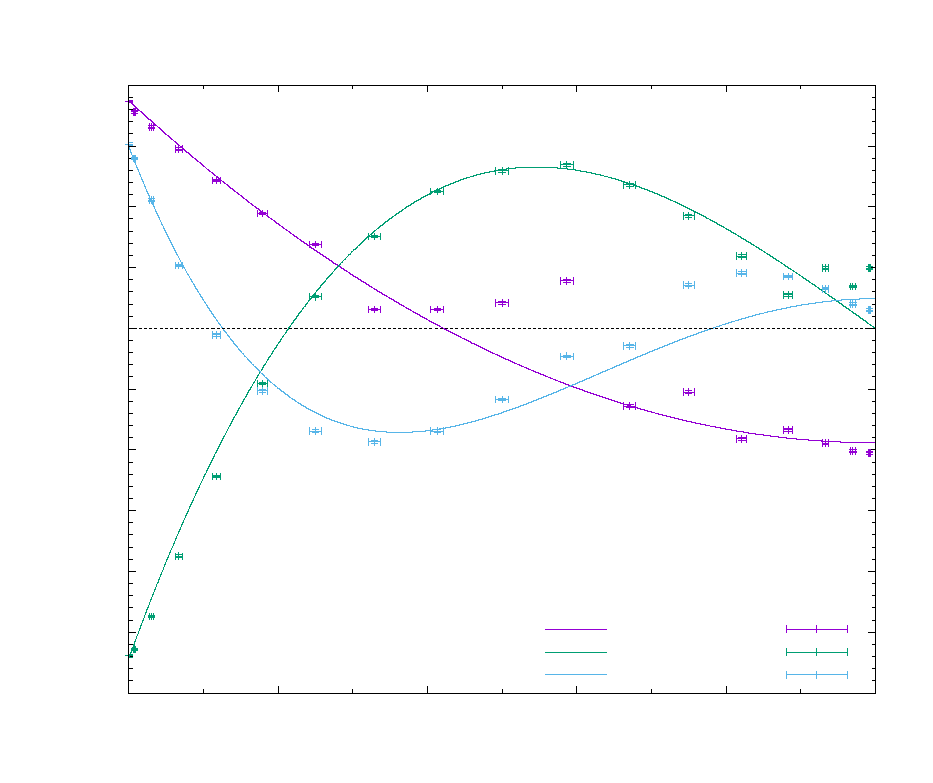
\includegraphics[width={432.00bp},height={360.00bp}]{tv2a}}%
    \gplfronttext
  \end{picture}%
\endgroup
}
		    \caption{Zuordnung der Legendrepolynome}
		    \label{fig:tv1-2}
		    % \vspace{-1em}
		\end{figure}
		Es scheint, dass das Vorzeichen einiger Messungen falsch bestimmt waren, zum Beispiel: bei der zwei lila Punkten zwischen \num{-0.5} und \num{-0.4}. 

		Als Fit-Ergebnis haben wir:
		\begin{center}
			\begin{tabular}{lllll}
				\toprule
				Ordnung $l$ & Fit Variablen &&& $\chi^2_\text{red}$ \\
				\midrule
				$2$ &
				$A = \num{0.562(20)}$ & 
				$B = \num{-0.188(10)}$ &&  \num{140.555} \\
				$3$ &
				$C = \num{1.42(9)}$ &
				$D = \num{-0.88(8)}$ & & \num{296.633} \\
				$4$ &
				$E = \num{1.33(12)}$ &
				$F = \num{-1.08(12)}$ & 
				$G = \num{0.049(14)}$ & \num{224.661} \\
				\bottomrule
			\end{tabular}
		\end{center}
		Aus $\chi^2_\text{red} \gg 1$ sind die Kurveanpassungen eher schlecht. Das liegt vermutlich daran, dass die Messmethode eher ungenau ist. Da es um Schallwellen handelt, kommt es auch viele Störungen von außen. Die Wärme von der Hände könnte auch die Temperatur im Resonator über den Versuchsverlauf ändern, sodass die Schallgeschwindigkeit sich ändert. Es war auch während des Versuchs beobachtet, dass die Spannung sich mit der Zeit langsam geändert hat, ohne dass ich irgendwas gemacht hatte. 

		\pagebreak
		Wir vergleichen nun die erhaltene Ergebnissen. Um irgendwelche Skalierungsfaktor zu vermeiden, schauen wir die Verhältnisse zwischen die Variablen an. Der Fehler ist dann gegeben durch:
		\begin{align}
			\Delta \left(\frac{x}{y}\right) = \abs{\frac{x}{y}}\relquad{x,y}
		\end{align}
		\begin{center}
			\begin{tabular}{lrrr}
				\toprule
				Variable & Literatur & Experimentell & Bemerkung \\
				\midrule
				$\nicefrac{A}{B}$ & $-3$ & \num{-2.99(20)} & stimmen überein \\
				$\nicefrac{D}{C}$ & $\num{-0.6}$ & \num{-0.62(7)} & stimmen überein \\
				$\nicefrac{E}{F}$ & $\num{-1,16667}$ & \num{-1,23(18)} & stimmen überein \\
				$\nicefrac{E}{G}$ & $\num{11,6667}$ & \num{27(9)} & verträglich \\
				$\nicefrac{F}{G}$ & $\num{-10}$ & \num{22(7)} & verträglich \\
				\bottomrule
			\end{tabular}
		\end{center}
		Die Abweichungen sind vermutlich der oben beschriebenen Fehlerquellen zufolge. 

		Die Nullstellen der Fit werden mit WolframAlpha berechnet. Dabei ist die Fehler aus zeitlichen Gründen vernachlässigt.
		\begin{center}
			\begin{tabular}{lrrrr}
				\toprule
				$l$ & $2$ & $3$ & $4$ & $4$ \\
				Manuell/\si{\degree} & \num{125.3(7)} & \num{141.2(7)} & \num{110.2(7)} & \num{152.7(7)} \\
				Fit/\si{\degree}     & \num{125.34}   & \num{141.93}   & \num{102.69}   & \num{150.92} \\
				\bottomrule
			\end{tabular}
		\end{center}
		Sie stimmen also überein bzw. für $\SI{110.2(7)}{\degree}$ verträglich.


	\subsection{Teilversuch 2b: Bestimmung der $l$-Quantenzahl durch zweidimensionale Darstellung der Messergebnisse als Orbitalform}
		\begin{figure}[!ht]
			\begin{subfigure}{0.3\textwidth}
				\centering
				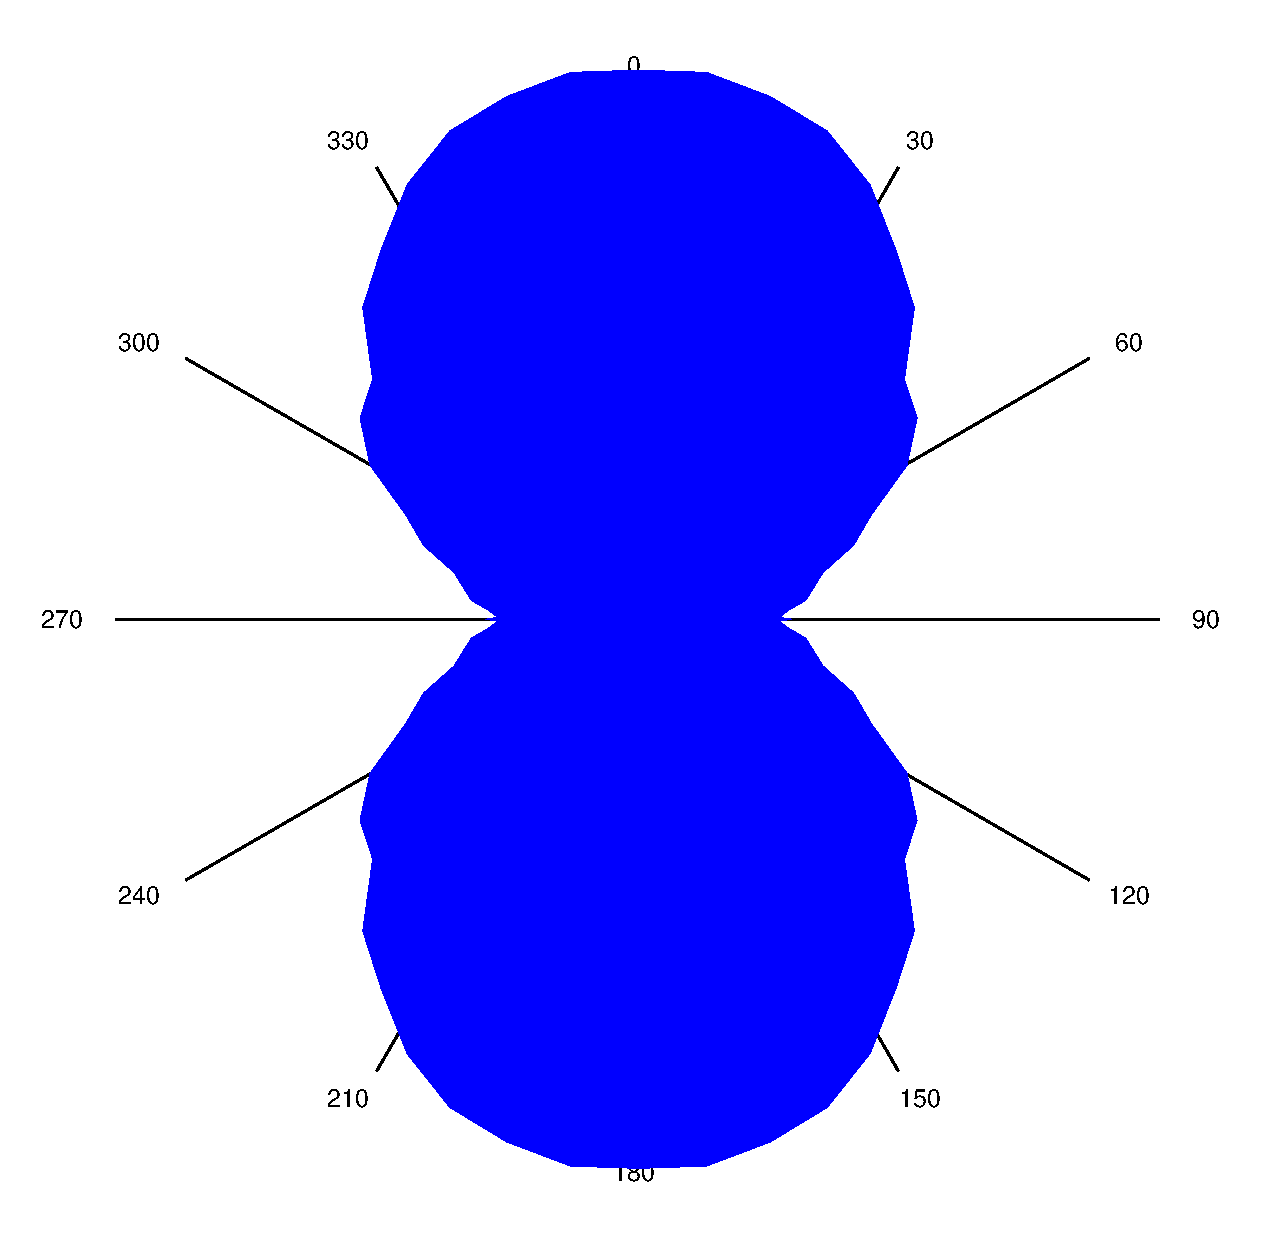
\includegraphics[width=\textwidth]{images/tv2b-180deg-peak1-angle.eps}
				\caption{$l = 1, m=0$}
				% \vspace{0.5\baselineskip}
				\label{fig:tv2b-1}
			\end{subfigure}
			\begin{subfigure}{0.3\textwidth}
				\centering
				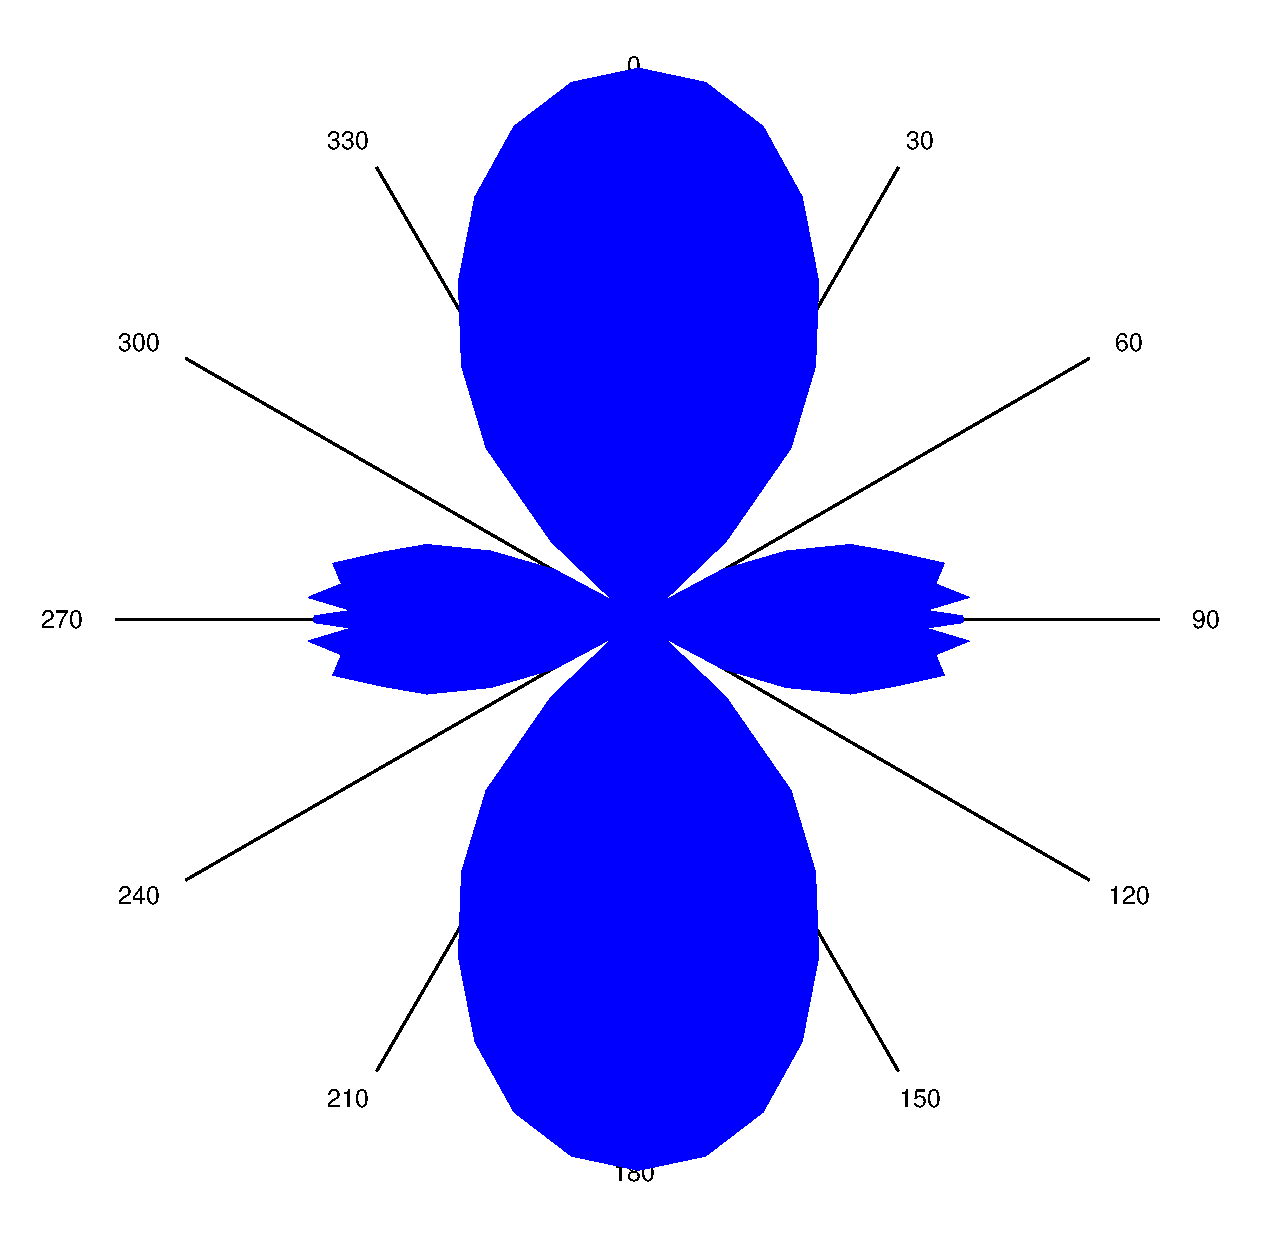
\includegraphics[width=\textwidth]{images/tv2b-180deg-peak2-angle.eps}
				\caption{$l = 2, m=0$}
				% \vspace{0.5\baselineskip}
				\label{fig:tv2b-2}
			\end{subfigure}
			\begin{subfigure}{0.3\textwidth}
				\centering
				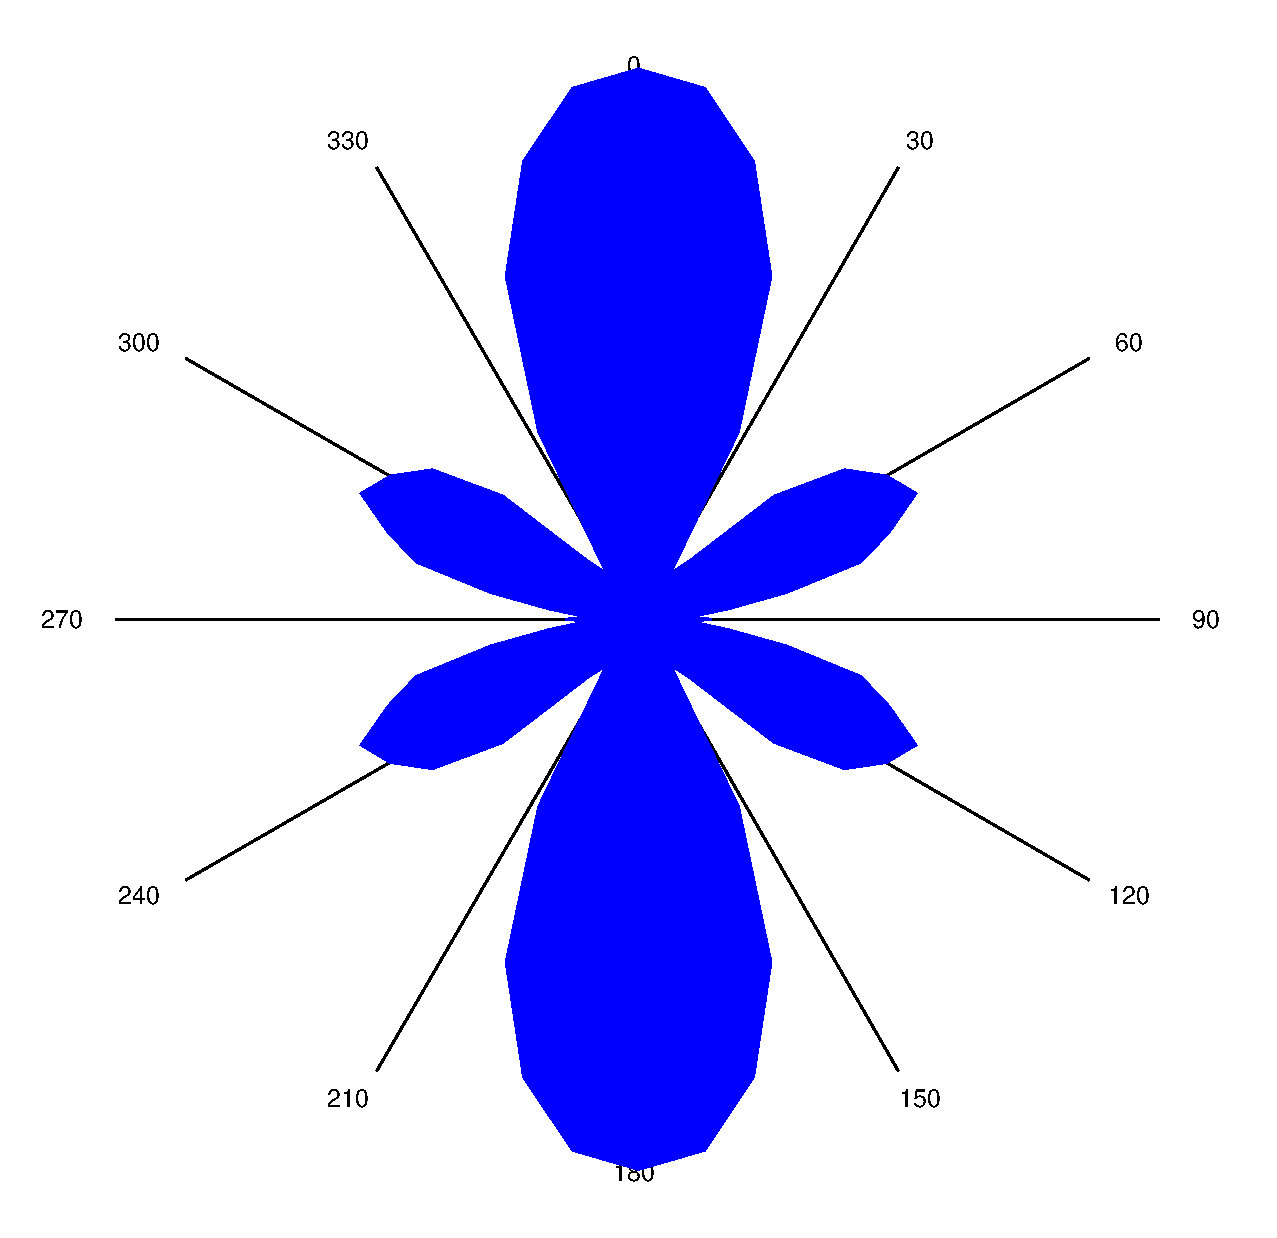
\includegraphics[width=\textwidth]{images/tv2b-180deg-peak3-angle.eps}
				\caption{$l = 3, m=0$}
				% \vspace{0.5\baselineskip}
				\label{fig:tv2b-3}
			\end{subfigure}
		    \caption{Teilversuch 2b}
		\end{figure}
		Abweichungen z.b. bei Abbildung \ref{fig:tv2b-2} sind vermutlich wegen Störungen während der Messungen.

		Wie können die $l$-Quantenzahl bestimmen, indem wir die Anzahl der Nullstellen zahlen, wenn wir $\theta$ von \SI{0}{\degree} bis \SI{180}{\degree}. Die Anzahl der Nullstellen ist genau $l$.

		Andere Auswertungen siehe Laborprotokoll.



	
\section{Teilversuch 3: Aufnahme des Spektrums der Neon-Glimm\-ent\-la\-dung}
	


\resnum
% \newpage
\appendix
%  Bibliography
    \renewcommand*{\bibfont}{\raggedright}
    \urlstyle{sf}
    \hypersetup{urlcolor=gray}
    \printbibliography
% / Bibliography
\end{document}
